\usepackage{tikz}
\usepackage[utf8]{inputenc}
\usepackage{amsmath}
\usepackage{amsfonts}
\usepackage{amssymb}
\usepackage{stackrel}
%\usepackage{kpfonts}
\usepackage{amssymb, amsmath, amsbsy} 
\usepackage{makeidx}
\usepackage{graphicx}
\usepackage{multicol}
\usepackage{changepage}
\usepackage{float}
\usepackage{cite}
\usepackage{lipsum}
\usepackage{pstricks, caption}
\usepackage{url}
\usepackage[spanish, es-tabla]{babel}
\usepackage[shortlabels]{enumitem}
\usepackage{longtable,multirow,booktabs}
\usepackage{rotating}
\usepackage{caption}
\usepackage{multirow, array}
\usepackage{anyfontsize}
\usepackage{fix-cm}
\usepackage{calligra}
\usepackage{mathptmx}
\usepackage{caption}
\usepackage{fancyvrb}
%\usepackage{esvect}
\usepackage{xargs}
\usepackage{subfigure} 
\usepackage {titletoc}
\usepackage[T1]{fontenc}
%\usepackage[hyphens]{url}
\usepackage[breaklinks,colorlinks=true,linkcolor=blue,citecolor=red, urlcolor=blue]{hyperref}
\usepackage{flushend}
\usepackage{amsmath,amsthm,amssymb}

\documentclass[13,twocolumn,letterpaper]{article}
    \usepackage[spanish,english]{babel}
    \usepackage[utf8x]{inputenc}
    \usepackage[T1]{fontenc}
    \usepackage[a4paper,top=3cm,bottom=2cm,left=3cm,right=3cm,marginparwidth=1.75cm]{geometry}
    \usepackage{amsmath}
    \usepackage[colorinlistoftodos]{todonotes}
    \usepackage[colorlinks=true, allcolors=blue]{hyperref}
    \usepackage{float}
    
    
 \spanishdecimal{.}
\renewcommand{\figurename}{\textbf{Figura}}
\renewcommand{\tablename}{\textbf{Tabla}}
\renewcommand{\refname}{Bibliografía}
\renewcommand{\abstractname}{\large\textbf{Resumen}}
\renewcommand{\contentsname}{Contenido}
\renewcommand{\partname}{Parte}
\renewcommand{\appendixname}{Apéndice}
\renewcommand{\sin}{sen}	
\newenvironment{Figure}{\par\medskip\noindent\minipage{\linewidth}}{\endminipage\par\medskip}

    
    \title{
    		%\vspace{-1in} 	
    		\usefont{OT1}{bch}{b}{n}
    		\normalfont \normalsize \textsc{INSTITUTO POLITÉCNICO NACIONAL \\ 
    		ESCUELA SUPERIOR DE FISICA Y MATEMATICAS \\
    		ACADEMIA DE FÍSICA EXPERIMENTAL} \\ 
    		FÍSICA IV: LABORATORIO DE ÓPTICA. \\[10pt]
    		\huge Práctica IX:\\
  Difracción de Fraunhofer por Doble Rendija y Red de Difracción.\\
    }
    
    \usepackage{authblk}
    \author[0]{Alumno: Flores Rodriguez Jaziel David \\
    Boleta: 2014030429 \\
    Profesor: Dr. Janos Zsargo\\
    Grupo: 4FV2-B \\
            }
    \begin{document}
    
    \maketitle
   
    \selectlanguage{spanish}
    
    \section*{Resumen}
Determinar el ancho de la doble rendija del experimento de Young a partir del patrón de  difracción. Determinar  la  longitud  de  onda  del  láser  a  partir  del  patrón  de difracción producido por la red de difracción.\\ 

\section*{Introducción}

\textbf{Difracción}: es  un  fenómeno  característico  de  lasondasque  se  basa  en  la desviación  de  estas  al  encontrar  un  obstáculo  o  al  atravesar  una  rendija.  La difracción  ocurre  en  todo  tipo  de  ondas,  desde  ondas sonoras,  ondas  en  la superficie de un fluido y ondas electromagnéticas como laluz visibley lasondas de radio.\\

También sucede cuando un grupo de ondas de tamaño finito se propaga; por ejemplo,   por   causa   de   la   difracción,   el   hazcolimadode   ondas   de   luz   de unláserdebe finalmente divergir en un rayo más amplio a una cierta distancia del emisor. \\

\textbf{Difracción  de  Fraunhofer}: también difracción  del  campo  lejano es  un  patrón  de difracción de  una  onda electromagnética  cuya  fuente  (al  igual  que  la pantalla)  se encuentran  infinitamente  alejadas del  obstáculo,  por  lo que  sobre  éste  y  sobre  la pantalla incidiránondas planas.\\

Una  forma  práctica  de  lograr  la  difracción  de Fraunhofer  en  condiciones  de laboratorio  es  utilizandolentes  convergentes  y  divergentespara  lograr  el  campo lejano y lasondas planas.

 \begin{figure}[h]
	\centering
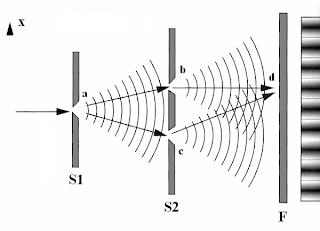
\includegraphics[width=\linewidth]{Fig91.png}
	\label{fig:fig3}
\end{figure}
 
 Red  de  difracción: unared  de  difracciónes  uncomponente  ópticocon  un  patrón regular, que divide (difracta) la luz en varios haces de luz que viajan en diferentes direcciones.\\
 
 Las direcciones de esos haces de luz dependen del espaciado de la red y de lalongitud de ondade la luz incidente, de modo que la red actúa como un elemento dispersivo.Un ejemplo de red de difracción que está al alcance de cualquiera es un CD-ROM. \\
 
 Puede usarse para demostrar el efecto de la difracción haciendo incidir sobre él luz solar y recogiendo está en una pared.Para el caso de un sistema formado por dos rendijas de anchura “b” cada una y separadas una distancia “h”. Suponiendo que la distancia a la pantalla es infinita de forma que los rayos difractados por cada rendija son paralelos entre sí.\\ 
 
 Para  un  punto  sobre  la  pantalla  donde  interfieren  estos  dos  rayos  enuna dirección $\theta$, la diferencia de camino entre los dos rayos es hsen$\theta$.\\


\begin{figure}[h]
	\centering
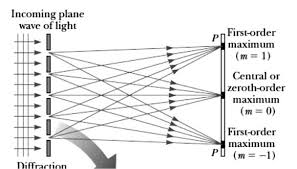
\includegraphics[width=\linewidth]{figgg.jpg}
	\label{fig:fig4}
\end{figure}

Así  todas   las   ondas   llegarán   en   fase   a   tal   punto   e   interferirán constructivamente para generar un máximo (una zona de brillo) si la diferencia de recorrido entre ellas esigual a la longitud de onda, o a un múltiplo de esa magnitud. La diferencia de recorrido entre ondas adyacentes es dsen($\theta$), por lo tanto, habrá un máximo donde la luz que proviene de todas las rendijas interfiere constructivamente a los ángulos:\\

                  $dsenθ = m\lambda$, donde m=0,-1,+1,-2,+2, ...\\ 
                  
El número m se conoce como número de orden, y cuando vale 0 se tiene la franja de brillo central que se lellama de orden máximo cero. Luego la franja de brillo siguiente a cada lado se produce cuando m = 1 o -1, y esentonces la franja de primer orden máximo.\\

De la misma forma se denominan el resto de las franjas de brilloque le siguen a cada lado (segundo orden máximo, tercer orden máximo y así sucesivamente)

\section*{Desarrollo Experimental.}

\subsection*{Experimento 1}
Se nos da un láser en el cual se le coloca un placa que contiene rendijas pequeñas en frente de él, luego procedimos a medir el la distancia del láser hasta la pantalla (pared) para obtener“D”.\\

La placa hará que se difracte el láser así en la pantalla tendremos varios “láseres” medimos la distancia que están separados a partir del láser central para obtener “y”.\\

Se repite el método II con otro 2 tipos de placas en nuestro caso cada placa tenia rendijillas de 300 líneas/mm, 80 líneas/mm y 100 líneas/mm \\

Con la ecuación anterior se calculará la longitud de onda que tiene el láser, el ángulo de desviación está dada por arctan($\frac{y}{D}$) \\


\subsection*{Experimento 2}

Se hace lo mismo que en el experimento 1 solo que ahora nos dan un soporte con una placa que tiene rendijas como las que uso Young en su experimento cada rendijilla tiene diferente líneas/mm así que calcularemos eso haciendo un promedio de cada resultado que nos da la ecuación anterior.\\


\section*{Datos y Resultados Obtenidos}
\subsection*{Experimento 1}
Para la placa de 80 lineas/mm

\begin{table}[h]
    \centering
    \begin{tabular}{|| c | c | c | c ||}
\hline 
D (cm) & \textbf{d}$(cm)$ & Y (cm) & $\mathbf{\lambda}$ $(n m)$ \\ \hline
$\frac{1}{80}$ & 103 & 5,2 & 504,426 \\ \hline
$\frac{1}{80}$ & 10310 & 10,7434 & 434,976 \\ \hline
    \end{tabular}
    \label{tab:my_label}
\end{table}

Placa de 300 lineas/mm

\begin{table}[h]
    \centering
    \begin{tabular}{|| c | c | c | c ||}
\hline 
D (cm) & \textbf{d}$(cm)$ & Y (cm) & $\mathbf{\lambda}$ $(n m)$ \\ \hline
$\frac{1}{300}$ & 103 & 19,5 & 635,8049 \\ \hline
$\frac{1}{300}$ & 103 & 41 & 625,3154 \\ \hline
    \end{tabular}
    \label{tab:my_label}
\end{table}

Placa de 100 líneas/mm
    
\begin{table}[h]
    \centering
    \begin{tabular}{|| c | c | c | c ||}
\hline 
D (cm) & \textbf{d}$(cm)$ & Y (cm) & $\mathbf{\lambda}$ $(n m)$ \\ \hline
$\frac{1}{100}$ & 103 & 6,5 & 649,071 \\ \hline
$\frac{1}{100}$ & 103& 13,1 & 640,713 \\ \hline
    \end{tabular}
    \label{tab:my_label}
\end{table}
Placa de 600 líneas/mm

\begin{table}[h]
    \centering
    \begin{tabular}{|| c | c | c | c ||}
\hline 
D (cm) & \textbf{d}$(cm)$ & Y (cm) & $\mathbf{\lambda}$ $(n m)$ \\ \hline
$\frac{1}{600}$ & 103 & 42 & 632,091 \\ \hline
$\frac{1}{600}$ & 103 & 118,2 & 630,086  \\ \hline
    \end{tabular}
    \label{tab:my_label}
\end{table}
\pagebreak
\subsection*{Experimento 2}

Primer Rendija \\

\begin{table}[h]
    \centering
    \begin{tabular}{|| c | c | c | c | c ||}
\hline 
m & D (cm) & y (cm) & $\mathbf{\lambda}$ (nm) & d(nm) \\ \hline
1 & 159.5 & 0.6 & 633 & 168273.69 \\ \hline
-1 & 159.5 & 0.42 & 633 & 240390.11 \\ \hline
 \end{tabular}
    \label{tab:my_label}
\end{table}

Segunda Rendija \\

\begin{table}[h]
    \centering
    \begin{tabular}{|| c | c | c | c | c ||}
\hline 
m & D (cm) & y (cm) & $\mathbf{\lambda}$ (nm) & d(nm) \\ \hline
1 & 159.5 & 0.335 & 633 & 301384.24 \\ \hline
-1 & 159.5 & 0.41 & 633 & 246253.25 \\ \hline
 \end{tabular}
    \label{tab:my_label}
\end{table}

Tercera Rendija \\

\begin{table}[H]
    \centering
    \begin{tabular}{|| c | c | c | c | c ||}
\hline 
m & D (cm) & y (cm) & $\mathbf{\lambda}$ (nm) & d(nm) \\ \hline
1 & 159.5 & 0.135 & 633 & 747878.04 \\ \hline
-1 & 159.5 & 0.145 & 633 & 696300.28 \\ \hline
 \end{tabular}
\end{table}

I. Obtengamos los promedios de  $\mathbf{\lambda}$.\\

Para la primer:\\

$\mathbf{\lambda}=\frac{504,426+434,976}{2}=469,701$\\
\\
Para la segunda: \\

$\mathbf{\lambda}=\frac{635,8048+625,3154}{2}=630,56015$\\
\\
Para la tercer:\\

$\mathbf{\lambda}=\frac{649,071+640,713}{2}=644,892$\\
\\
Para la cuarta: \\

$\mathbf{\lambda}=\frac{632,091+630,086}{2}=631,0885$\\
\\
En general, el valor que se debió obtener es de 632,8. Así que de los promedios obtenidos aquí, soloen la primer tabla se discrepa de manera considerable, por tanto solo se calculará el error porcentualen ese caso, teniendo así  
\\
\\
$e\%=\frac{|632,8−469,701|}{632,8}\times(100) = 25,7741\%$
\\  

II.Primer tabla\\

$d=\frac{168373,69+240390,11}{2}=204331,9$\\
\\
\\
\\
Segunda tabla\\

$d=\frac{301384.24+246253.25}{2}=270887.2$\\
\\
Tercer tabla\\

$d=\frac{747878.04+696300.28}{2}=722089.1$\\

\\
\section*{Conclusiones}

Como se vio en la introducción teórica se necesita que la distancia entre la fuente y la pantalla debe de sermuy grande a comparación de la separaciones de máximos/mínimos de la luz, pues es necesario para lasaproximaciones   que   se   hicieron   en   el   desarrollo   de   la   formula,   además   la   luz   se   pueda   difractar   nonecesariamente con un material específico si no que con solo un material con opaco y con pequeños agujerosse pueden simular rendijillas.
 


\nocite{Hecht}\nocite{Rossi}\nocite{Sears}\nocite{Born}\nocite{Tipler}\nocite{Feynman}\nocite{Res}
\bibliography{miBiblio.bib}
\bibliographystyle{plain}
\end{document}